\documentclass[
  bibliography=totoc,     % Literatur im Inhaltsverzeichnis
  captions=tableheading,  % Tabellenüberschriften
  titlepage=firstiscover, % Titelseite ist Deckblatt
]{scrartcl}

\usepackage[ngerman]{babel} 
\usepackage[utf8]{inputenc}
\usepackage[T1]{fontenc} 
\usepackage{lmodern}
\usepackage{setspace}
\usepackage{wrapfig} %Für Bilder
\usepackage{xcolor} %Farbe

\usepackage[activate={true,nocompatibility},final,tracking=true,kerning=true,spacing=true,factor=1100,stretch=10,shrink=10]{microtype}
% activate={true,nocompatibility} - activate protrusion and expansion
% final - enable microtype; use "draft" to disable
% tracking=true, kerning=true, spacing=true - activate these techniques
% factor=1100 - add 10% to the protrusion amount (default is 1000)
% stretch=10, shrink=10 - reduce stretchability/shrinkability (default is 20/20)


%\usepackage{scrpage2}

\usepackage{amssymb} % Mathe Symbole
\usepackage{amsmath} % Mathe
\usepackage{mathtools} % Erweiterungen für amsmath
\usepackage{esvect} %Für vektoren

\usepackage{setspace} % Fuer eine Liste mit Abk.
\usepackage{listings} % Um Code schoener aussehen zu lassen

% Zahlen und Einheiten
\usepackage[
  locale=DE,                   % deutsche Einstellungen
  separate-uncertainty=true,   % immer Fehler mit \pm
  per-mode=symbol-or-fraction, % / in inline math, fraction in display math
]{siunitx}

% chemische Formeln
\usepackage[
  version=4,
  math-greek=default, % ┐ mit unicode-math zusammenarbeiten
  text-greek=default, % ┘
]{mhchem}

% richtige Anführungszeichen
\usepackage[autostyle]{csquotes}

% schöne Brüche im Text
\usepackage{xfrac}

% Standardplatzierung für Floats einstellen
\usepackage{float}
\floatplacement{figure}{htbp}
\floatplacement{table}{htbp}


%keine Floats in anderen Sectionen
\usepackage{placeins}

\let\Oldsection\section
\renewcommand{\section}{\FloatBarrier\Oldsection}

\let\Oldsubsection\subsection
\renewcommand{\subsection}{\FloatBarrier\Oldsubsection}

\let\Oldsubsubsection\subsubsection
\renewcommand{\subsubsection}{\FloatBarrier\Oldsubsubsection}

% Seite drehen für breite Tabellen: landscape Umgebung
\usepackage{pdflscape}

% Captions schöner machen.
\usepackage[
  labelfont=bf,        % Tabelle x: Abbildung y: ist jetzt fett
  font=small,          % Schrift etwas kleiner als Dokument
  width=0.9\textwidth, % maximale Breite einer Caption schmaler
]{caption}
% subfigure, subtable, subref
\usepackage{subcaption}

% Grafiken können eingebunden werden
\usepackage{graphicx}
% größere Variation von Dateinamen möglich
\usepackage{grffile}

% schöne Tabellen
\usepackage{booktabs}

% Verbesserungen am Schriftbild (scheint zu Fehlern zu führen)
%\usepackage{microtype}

% Literaturverzeichnis
\usepackage[
  backend=biber,
]{biblatex}
% Quellendatenbank
\addbibresource{lit.bib}
\addbibresource{programme.bib}

\usepackage{breakcites}

% Hyperlinks im Dokument
\usepackage[
  unicode,        % Unicode in PDF-Attributen erlauben
  pdfusetitle,    % Titel, Autoren und Datum als PDF-Attribute
  pdfcreator={},  % ┐ PDF-Attribute säubern
  pdfproducer={}, % ┘
]{hyperref}

% erweiterte Bookmarks im PDF
\usepackage{bookmark}

%erweiterte Aufzählungen
\usepackage{paralist}

% Trennung von Wörtern mit Strichen
\usepackage[shortcuts]{extdash}

\author{%
  David Rolf%
  \texorpdfstring{%
    \\%
    \href{mailto:david.rolf@tu-dortmund.de}{david.rolf@tu-dortmund.de}
  }{}%
  \texorpdfstring{\and}{, }%
  Jonah Blank%
  \texorpdfstring{%
    \\%
    \href{mailto:jonah.blank@tu-dortmund.de}{jonah.blank@tu-dortmund.de}
  }{}%
}
%\publishers{TU Dortmund – Fakultät Physik}

% Ableitungen mit \diff
\newcommand{\diff}{\mathop{}\!\mathrm{d}}

% mache . zu einem aktiven Zeichen im Mathemodus 
\mathcode`\.="8000 
% Dann kommt die Umdefinition des Dezimalpunktes 
\begingroup\lccode`~=`. 
  \lowercase{\endgroup\def~}#1{\mathrm{#1}} 
\subject{V46}
\title{\texorpdfstring{Faraday-Effekt}{}}
\date{
\begin{center}
	 Durchführung: 27.01.2020 \hspace{3em} Abgabe: 20.02.2020\\
	 \begin{figure}
	 \centering
	 
\includegraphics[scale=0.2]{content/images/tu.jpg}
	 \end{figure}
	 Fakultät Physik
\end{center}
}

\begin{document}
	\maketitle
	\newpage
	\tableofcontents
	\newpage
	
\section{Zielsetzung}
\label{sec:Zielsetzung}

Ziel des Versuchs ist es die Wärmekapazität verschiedener Metalle zu ermitteln, um zu bestimmen, ob die Schwingungen von Atomen im Festkörper den Gesetzen der klassischen Physik oder Quantenmechanik folgen.
	
\section{Theorie}
\label{sec:Theorie}

\subsection{Wärmekapazität}
Die Molwärme $C$ eines Körpers bezeichnet seine Proportionalität zwischen der aufgenommenen Wärme $dQ$ und der Veränderung der Temperatur $dT$.
\begin{equation}
C = \frac{dQ}{dT} \label{eq:C}
\end{equation}
Man unterscheidet dabei die spezifische Wärmekapazität bei konstantem Druck $C_\text{p}$ und die bei konstantem Volumen $C_\text{V}$.\newline
Der erste Hauptsatz der Thermodynamik für die Innere Energie $U$ eines Systems lautet \[dU=dQ-pdV\]
für $V = const$ folgt $dV = 0$ und damit $dU = dQ$.
Damit ergibt sich für die Wärmekapazitäten:
\begin{equation}
C_\text{V} = \left(\frac{dU}{dT}\right)_\text{V} \label{eq:CV}
\end{equation}
und 
\begin{equation}
C_\text{p} = \left(\frac{dQ}{dT}\right)_\text{p} \label{eq:Cp}
\end{equation}
Das Verhältnis zwischen diesen beiden lässt sich durch
\begin{equation}
C_\text{V}= C_\text{p} - 9,\alpha^2\kappa V_0T \label{eq:CpCV}
\end{equation}
beschreiben\cite{V201}, wobei $\alpha$ der Ausdehnungskoeffizient und $\kappa$ die Kompressibilität des Stoffes ist.
$V_0$ ist das Molvolumen und kann als 
\begin{equation*}
V_0 = \frac{M}{\rho}
\end{equation*}
mit der molaren Masse $M$ und der Dichte $\rho$ geschrieben werden.
Die Wärmekapazität $c_\text{g}m_\text{g}$ eines Kalorimeters lässt sich durch die Mischtemperatur $T_\text{M}$ von zwei Wassermengen mit verschiedenen Temperaturen $T_\text{x}$ und $T_\text{y}$ und den Massen $m_\text{x}$ und $m_\text{y}$, sowie die Wärmekapazität des Wassers $c_\text{W}\approx \SI{4,18}{\joule\per\gram\per\kelvin}$ bestimmen\cite{V201}:
\begin{equation}
c_\text{g}m_\text{g} =\frac{ c_\text{w}m_\text{y}(T_\text{y}-T_\text{m})- c_\text{w}m_\text{x}(T_\text{m}-T_\text{x})}{(T_\text{m}-T_\text{x})} \label{eq:cgmg}
\end{equation}
Damit lässt sich auch die spezifische Wärmekapazität einer Probe $c_\text{k}$ bestimmen als \cite{V201}
\begin{equation}
c_\text{k} =\frac{( c_\text{W}m_\text{W}+ c_\text{g}m_\text{g})(T_\text{m}-T_\text{W})}{m_\text{k}(T_\text{k}-T_\text{m})}. \label{eq:ck}
\end{equation}
Daraus und mit Gleichung \eqref{eq:CpCV} folgt für $C_\text{V}$: 
\begin{equation}
C_\text{V}= c_\text{k}M - 9,\alpha^2\kappa \frac{M}{\rho}T. \label{eq:ckCV}
\end{equation}
\subsection{Dulong-Petit in der klassischen Physik}
Laut dem Dulong-Petitschen Gesetz beträgt die spezifische Wärmekapazität $C_\text{V}$ unabhängig von den Eigenschaften des Körpers den Wert \[C_\text{V}=3R,\]
wobei \begin{equation}
R = N_\text{A} k_\text{B} \label{eq:R}
\end{equation}
\begin{equation*}= \SI{8,314}{\joule\per\mol\per\kelvin}
\end{equation*} ist.
Aus der klassischen Sichtweise lässt sich dies dadurch errechnen, dass die Atome in einem Festkörper sich nur in Form 
von Schwingungen und damit wie der bekannte harmonischer Oszillator bewegen können.
Die mittlere innere Energie beträgt in diesem Fall
\begin{equation}
\langle U \rangle = \langle E_\text{pot} \rangle + \langle E_\text{kin}\rangle= 2 \langle E_\text{kin} \rangle \label{eq:U}
\end{equation}
Da außerdem nach dem Äquipartitionstheorem ein Atom eine mittlere kinetische Energie
\begin{equation*}
\langle E_\text{kin}\rangle = \frac{1}{2}k_\text{B}T
\end{equation*}
pro Freihatsgrad f besitzt, folgt aus Gleichung \eqref{eq:U} eine mittlere Gesamtenergie
\begin{equation}
\langle U \rangle= k_\text{B}T. \label{eq:U2}
\end{equation}
Betrachtet man nun ein $\si{\mol}$ Atome muss das dies mit der Avogradokonstanten $N_\text{A} = 6,2 x10^{23}$ multipliziert werden.
Mit Gleichung \eqref{eq:R} und unter Berücksichtigung, dass jedes Atom drei Freiheitsgrade der Rotation besitzt folgt schließlich
\begin{equation}
\langle U \rangle = 3RT \label{eq:U3}
\end{equation}
und somit aus Gleichung \eqref{eq:CV}
\begin{equation}
C_V = 3R \label{eq:CV2}
\end{equation}
\subsection{Dulong-Petit in der Quantenmechanik}
Bei hohen Temperaturen trifft diese spezifische Wärmekapazität auf alle festen Elemente zu, sie werden jedoch bei geringen Temperaturen beliebig klein. Da beim klassischen Ansatz davon ausgegangen wird, dass Energien in beliebig kleinen Beträgen aufgenommen und abgegeben werden können, kann dieser das Phänomen der geringen Kapazität nicht erklären.\newline
In der Quantentheorie aber wird davon ausgegangen, dass Energie nur gequantelt, also in diskreten Beträgen aufgenommen und abgegeben wird. \newline Das Atom, also der harmonisch mit der Frequenz $\omega$ schwingende Oszillator kann deshalb seine Gesamtenergie nur um 
\begin{equation}
\Delta U=\hbar\,\omega \label{eq:deltaU}
\end{equation}
oder Vielfache davon verändern.
Daher kann man nicht mehr mit einer lineare $T$-Abhängigkeit ausgegangen, sondern muss die Boltzmann-Verteilung berücksichtigt werden.\newline
So erhält man als neue mittlere Gesamtenergie pro Freiheitsgrad \cite{V201}
\begin{equation*}
\langle U \rangle = \frac{\hbar\,\omega}{e^{\frac{\hbar\,\omega}{k_\text{B}T}-1}}
\end{equation*}
und für die Gesamtenergie von einem $\si{\mol}$ Atomen
\begin{equation}
\langle U \rangle = \frac{3N_\text{A}\hbar\,\omega}{e^{\frac{\hbar\,\omega}{k_\text{B}T}-1}}. \label{eq:U4}
\end{equation}
Für $T\rightarrow0$ geht auch $\langle U \rangle$ gegen null und beschreibt somit die abweichenden $C_\text{V}$-Werte für geringe Temperaturen.
Für hohe Temperaturen wird $\langle U \rangle \approx 3N_\text{A}k_\text{B}T= 3RT$ wie im klassischen Fall.
	\section{Aufbau}
\label{sec:Aufbau}

In Abbildung \ref{fig:schema} ist der Versuchsaufbau zur Beobachtung des Zeeman-Effekts einer Cadmium(Cd)-Lampe schematisch dargestellt.
Diese wird in das Magnetfeld eines Elektromagneten eingebracht und die entstehenden Emissionslinien transversal zum Magnetfeld durch eine Anordnung von Linsen kollimiert. Die parallelen Strahlen fallen auf ein Geradsichtprisma und werden so entsprechend ihrer Wellenlänge aufgespalten. Durch einen Polarisationsfilter und einen Einzelspalt werden die zu untersuchenden Spektrallinien extrahiert und mittels Linsen auf eine Lummer-Gehrcke-Platte abgebildet. Das entstehende Interferenzmuster wird mithilfe einer Digitalkamera aufgenommen.

\begin{figure}
\centering
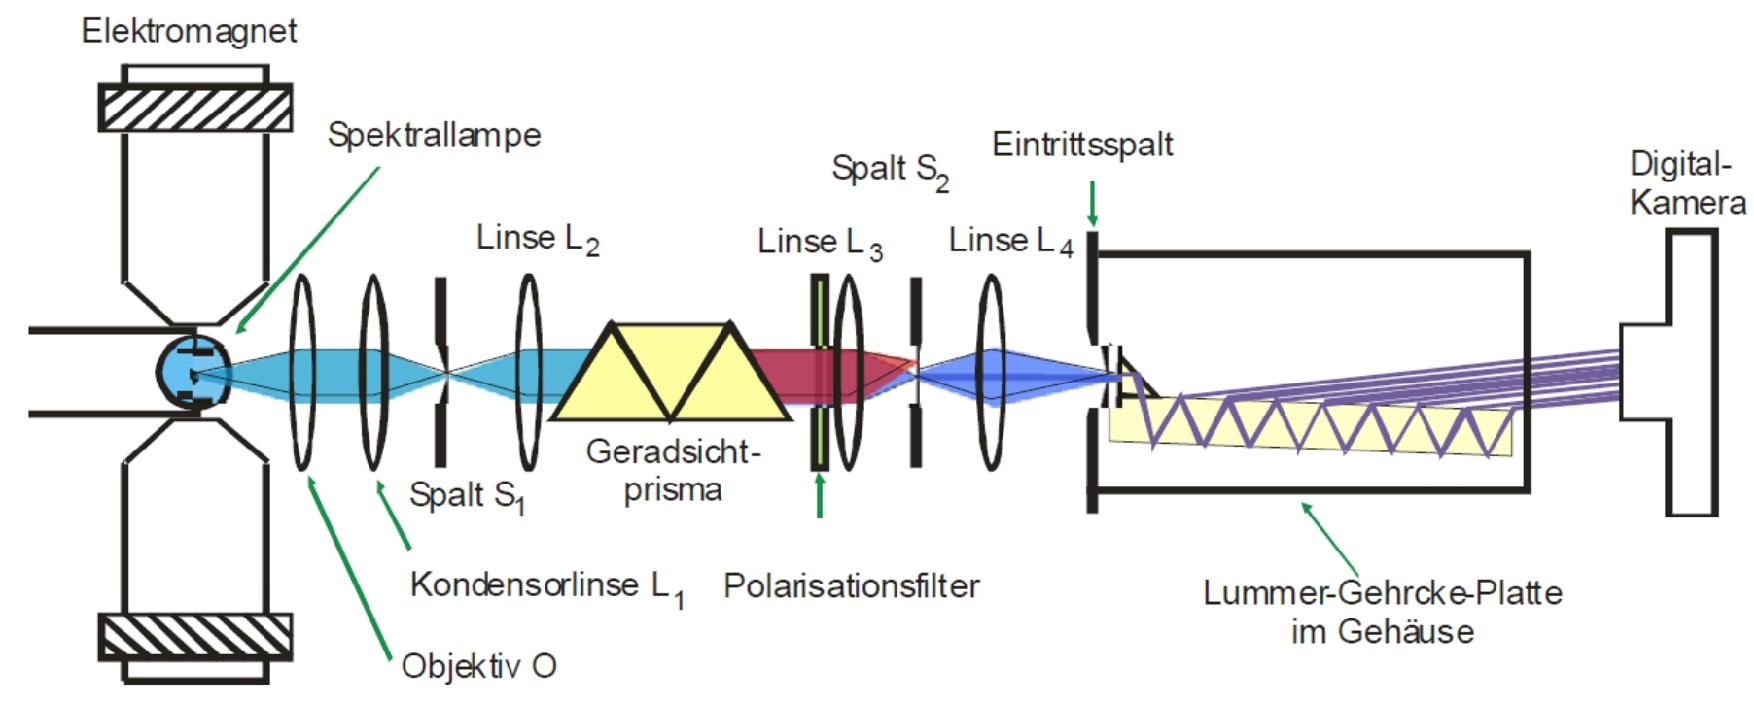
\includegraphics[width=0.8\textwidth]{build/schema.pdf}
\caption{Schematischer Aufbau zur Betrachtung des normalen und anormalen Zeeman-Effekts im Cadmium-Spektrum.\cite{V27}}
\label{fig:schema}
\end{figure}


%◘
	\section{Durchführung}
\label{sec:Durchführung}

Während allen Versuchen wird das Luftkissen eingeschaltet.
Nach jedem Messvorgang wird das externe Magnetfeld abgeschaltet, um die Spulen nicht zu überlasten.

\subsection{Messung über Gravitation} 

Die Stange wird mit der Masse in den Stiel an der Billardkugel gesteckt.
Es wird für zehn verschiedene Abstände der Masse zur Kugel die Stromstärke $I$ gemessen, bei der sich die Stange im Gleichgewicht befindet.

\subsection{Messung über Periodendauer}

Die Billardkugel wird am Stiel ausgelenkt und für zehn verschiedene Stromstärken wird die Periodendauer der resultieren Schwingung gemessen.

\subsection{Messung über Präzession}

Die Kugel wird in Rotation versetzt und aus der aufrechten Lage ausgelenkt.
Anschließend wird der weiße Punkt auf dem Stiel stroboskopisch mit einer Frequenz $\nu = \SI{5}{\hertz}$ beleuchtet. 
Sobald dieser stationär erscheint und damit die Frequenz des Stroboskops erreicht ist, wird das Magnetfeld eingeschaltet und für zehn verschiedene Stromstärken die Periodendauer der entstehenden Präzession gemessen.


	\newpage
	\section{Auswertung}
\label{sec:Auswertung}

Die Graphen werden sowohl mit Matplotlib \cite{matplotlib} als auch NumPy \cite{numpy} erstellt. Die Fehlerrechnung wird mithilfe von Uncertainties \cite{uncertainties} durchgeführt.

\subsection{Turbomolekularpumpe}

\subsubsection{Bestimmung des Saugvermögens $S$ über die Leckratenmessung}

Die Leckratenmessung wurde bei vier unterschiedlichen Gleichgewichtsdrücken $p_g$ durchgeführt. Dabei werden die gemessenen Zeiten $t_i$ mit der Formel für den Mittelwert
\[
\mu_t = \frac{1}{N}\sum_{i=1}^{N}t_i
\]
und dessen Standartabweichung
\[
\sigma_t = \frac{1}{N(N-1)}\sum_{i=1}^{N}(t_i-\mu_t)^2
\]
gemittelt zu
\begin{equation}
\bar{t} = \mu_t\pm \sigma_t\text{.} \label{eq:tQuer}
\end{equation} 
Dabei entspricht $N$ der Anzahl der durchgeführten Messungen pro Messreihe.
In den Tabellen \ref{tab:TL1} bis \ref{tab:TL4} sind die Messwerte und die zugehörigen Mittelwerte der jeweiligen Messreihen aufgelistet. Der Fehler des Druckes ergibt sich dabei aus der Ungenauigkeit der Messskala von $10\%$ \cite{V70}.\\
In den Abbildungen \ref{fig:TL1} bis \ref{fig:TL4} ist der Druck $p$ gegen die gemittelte Zeit $\bar{t}$ aufgetragen.
Die linearen Ausgleichsrechnungen der Form
\[
p_i(t) = a_it+b_i
\]
ergeben für $p_g = \SI{2e-4}{\milli\bar}$ die Parameter
\begin{align*}
a_.{TL1,1} &= \SI{4.4(1)e-4}{\milli\bar\per\second} \text{,}\\
b_.{TL1,1} &= \SI{0.6(8)e-4}{\milli\bar} \text{,}\\
a_.{TL1,2} &= \SI{4.7(1)e-4}{\milli\bar\per\second} \text{,}\\
b_.{TL1,2} &= \SI{-3.1(9)e-4}{\milli\bar} \text{,}\\
\end{align*}
für $p_g = \SI{1.4e-4}{\milli\bar}$
\begin{align*}
a_.{TL2,1} &= \SI{3.01(8)e-4}{\milli\bar\per\second} \text{,}\\
b_.{TL2,1} &= \SI{-0.7(9)e-4}{\milli\bar} \text{,}\\
a_.{TL2,2} &= \SI{3.30(4)e-4}{\milli\bar\per\second} \text{,}\\
b_.{TL2,2} &= \SI{-5.1(6)e-4}{\milli\bar} \text{,}\\
\end{align*}
für $p_g = \SI{1e-4}{\milli\bar}$
\begin{align*}
a_.{TL3,1} &= \SI{2.26(5)e-4}{\milli\bar\per\second} \text{,}\\
b_.{TL3,1} &= \SI{-1(1)e-4}{\milli\bar} \text{,}\\
a_.{TL3,2} &= \SI{2.46(5)e-4}{\milli\bar\per\second} \text{,}\\
b_.{TL3,2} &= \SI{-5(1)e-4}{\milli\bar} \text{,}\\
\end{align*}
und für $p_g = \SI{0.5e-4}{\milli\bar}$
\begin{align*}
a_.{TL4} &= \SI{0.676(4)e-4}{\milli\bar\per\second} \text{,}\\
b_.{TL4} &= \SI{0.43(3)e-4}{\milli\bar} \text{.}
\end{align*}
Der erste Index bezieht sich dabei auf die Messung bei gegebenem Gleichgewichtsdruck, der zweite Index bezieht sich auf die mögliche zweite Ausgleichsrechnung, bei der die erstsen drei Messwerte nicht mit berücksichtigt werden.
Mit Formel \eqref{eq:S2} ergibt sich für das Saugvermögen $S$
\begin{align*}
S_.{TL1,1} &= \SI{22(2)}{\litre\per\second} \text{,}\\
S_.{TL1,2} &= \SI{24(2)}{\litre\per\second} \text{,}\\
S_.{TL2,1} &= \SI{22(2)}{\litre\per\second} \text{,}\\
S_.{TL2,2} &= \SI{24(2)}{\litre\per\second} \text{,}\\
S_.{TL3,1} &= \SI{23(2)}{\litre\per\second} \text{,}\\
S_.{TL3,2} &= \SI{25(2)}{\litre\per\second} \text{,}\\
S_.{TL4}   &= \SI{14(1)}{\litre\per\second} \text{.}
\end{align*}
Das benötigte Volumen $V_.{TL}$ bestimmt sich dabei mit den Werten aus \ref{tab:V} zu:
\[
V_.{TL} = \dots = \SI{10.2(9)}{\litre}\text{.}
\]

\begin{table}
\centering
\caption{Die Messwerte der Leckratenmessung bei der Turborpumpe mit einem Gleichgewichtsdruck von $p_g = \SI{2e-4}{\milli\bar}$.}
\label{tab:tabTL1}
	\sisetup{table-format=1.2}
	\begin{tabular}{S[table-format=2.0]@{${}\pm{}$} S[table-format=1.1]S[table-format=2.2]S[table-format=2.2]S[table-format=2.2]S[table-format=2.2] @{${}\pm{}$} S[table-format=1.2]}
		\toprule
		\multicolumn{2}{c}{$p/10^{-4}\si{\milli\bar}$} & {$t_1/\si{\second}$} & {$t_2/\si{\second}$} & {$t_3/\si{\second}$} & \multicolumn{2}{c}{$\bar{t}/\si{\second}$} \\
		\midrule
		 6 & 0.6 & 1.20 & 1.01 & 0.99 & 1.07 & 0.07 \\
		10 & 1.0 & 2.29 & 2.29 & 2.09 & 2.22 & 0.07 \\
		20 & 2.0 & 4.75 & 4.87 & 4.64 & 4.75 & 0.07 \\
		30 & 3.0 & 7.08 & 7.15 & 7.00 & 7.08 & 0.04 \\
		40 & 4.0 & 9.31 & 9.31 & 9.13 & 9.25 & 0.06 \\
		50 & 5.0 & 11.24 & 11.27 & 11.23 & 11.25 & 0.01 \\
		60 & 6.0 & 13.17 & 13.37 & 13.11 & 13.22 & 0.08 \\
		\bottomrule
	\end{tabular}

\label{tab:TL1}
\end{table}

\begin{figure}
\centering
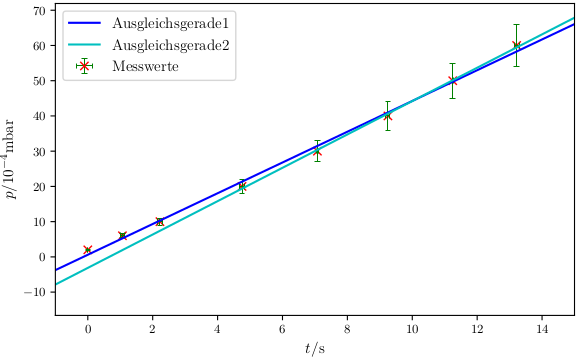
\includegraphics[width=\linewidth-70pt,height=\textheight-70pt,keepaspectratio]{content/images/TL1.png}
\caption{Der Druck $p$ in Abhängigkeit von der mittleren Zeit $\bar{t}$ bei der Leckratenmessung der Turbopumpe  mit $p_g = \SI{2e-4}{\milli\bar}$.}
\label{fig:TL1}
\end{figure}

\begin{table}
\centering
\caption{Die Messwerte der Leckratenmessung bei der Turborpumpe mit einem Gleichgewichtsdruck von $p_g = \SI{1.4e-4}{\milli\bar}$.}
\label{tab:tabTL2}
	\sisetup{table-format=1.2}
	\begin{tabular}{S[table-format=2.0] @{${}\pm{}$} S[table-format=1.1]S[table-format=2.2]S[table-format=2.2]S[table-format=2.2]S[table-format=2.2] @{${}\pm{}$} S[table-format=1.2]}
		\toprule
		\multicolumn{2}{c}{$p/10^{-4}\si{\milli\bar}$} & {$t_1/\si{\second}$} & {$t_2/\si{\second}$} & {$t_3/\si{\second}$} & \multicolumn{2}{c}{$\bar{t}/\si{\second}$} \\
		\midrule
		 6 & 0.6 & 2.06 & 2.15 & 2.13 & 2.11 & 0.03 \\
		10 & 1.0 & 3.64 & 3.81 & 3.81 & 3.75 & 0.06 \\
		20 & 2.0 & 7.57 & 7.45 & 7.49 & 7.50 & 0.04 \\
		30 & 3.0 & 10.68 & 10.75 & 10.62 & 10.68 & 0.04 \\
		40 & 4.0 & 13.66 & 13.80 & 13.88 & 13.78 & 0.06 \\
		50 & 5.0 & 16.62 & 16.86 & 16.76 & 16.75 & 0.07 \\
		60 & 6.0 & 19.48 & 19.66 & 19.66 & 19.60 & 0.06 \\
		\bottomrule
	\end{tabular}

\label{tab:TL2}
\end{table}

\begin{figure}
\centering
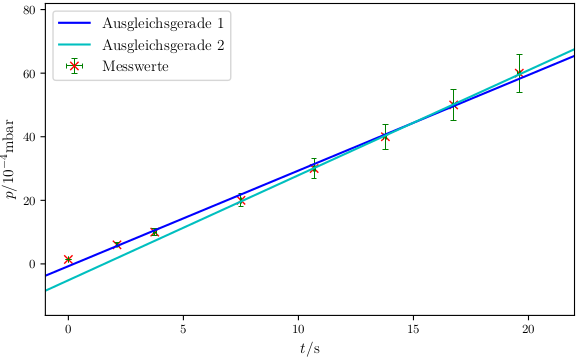
\includegraphics[width=\linewidth-70pt,height=\textheight-70pt,keepaspectratio]{content/images/TL2.png}
\caption{Der Druck $p$ in Abhängigkeit von der mittleren Zeit $\bar{t}$ bei der Leckratenmessung der Turbopumpe  mit $p_g = \SI{1.4e-4}{\milli\bar}$.}
\label{fig:TL2}
\end{figure}

\begin{table}
\centering
\caption{Die Messwerte der Leckratenmessung bei der Turborpumpe mit einem Gleichgewichtsdruck von $p_g = \SI{1e-4}{\milli\bar}$.}
\label{tab:tabTL3}
	\sisetup{table-format=1.2}
	\begin{tabular}{S[table-format=2.0] @{${}\pm{}$} S[table-format=1.1]S[table-format=2.2]S[table-format=2.2]S[table-format=2.2]S[table-format=2.2] @{${}\pm{}$} S[table-format=1.2]}
		\toprule
		\multicolumn{2}{c}{$p/10^{-4}\si{\milli\bar}$} & {$t_1/\si{\second}$} & {$t_2/\si{\second}$} & {$t_3/\si{\second}$} & \multicolumn{2}{c}{$\bar{t}/\si{\second}$} \\
		\midrule
		 1 & 0.1 & 0.00 & 0.00 & 0.00 & 0.00 & 0.00 \\
		 4 & 0.4 & 1.43 & 1.78 & 1.55 & 1.59 & 0.11 \\
		 8 & 0.8 & 3.66 & 4.14 & 3.93 & 3.91 & 0.14 \\
		20 & 2.0 & 9.54 & 10.17 & 9.93 & 9.88 & 0.19 \\
		30 & 3.0 & 14.28 & 14.46 & 14.59 & 14.44 & 0.09 \\
		40 & 4.0 & 18.39 & 18.84 & 18.92 & 18.72 & 0.17 \\
		50 & 5.0 & 22.50 & 22.85 & 23.00 & 22.78 & 0.15 \\
		60 & 6.0 & 26.23 & 26.69 & 26.68 & 26.53 & 0.16 \\
		70 & 7.0 & 29.88 & 30.37 & 30.38 & 30.21 & 0.17 \\
		\bottomrule
	\end{tabular}

\label{tab:TL3}
\end{table}

\begin{figure}
\centering
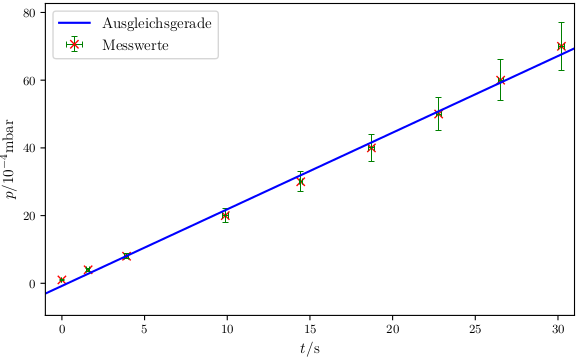
\includegraphics[width=\linewidth-70pt,height=\textheight-70pt,keepaspectratio]{content/images/TL3.png}
\caption{Der Druck $p$ in Abhängigkeit von der mittleren Zeit $\bar{t}$ bei der Leckratenmessung der Turbopumpe  mit $p_g = \SI{1e-4}{\milli\bar}$.}
\label{fig:TL3}
\end{figure}

\begin{table}
\centering
\caption{Die Messwerte der Leckratenmessung bei der Turborpumpe mit einem Gleichgewichtsdruck von $p_g = \SI{0.5e-4}{\milli\bar}$.}
\label{tab:tabTL4}
	\sisetup{table-format=1.2}
	\begin{tabular}{S[table-format=2.0] @{${}\pm{}$} S[table-format=1.1]S[table-format=2.2]S[table-format=2.2]S[table-format=2.2]S[table-format=2.2] @{${}\pm{}$} S[table-format=1.2]}
		\toprule
		\multicolumn{2}{c}{$p/10^{-4}\si{\milli\bar}$} & {$t_1/\si{\second}$} & {$t_2/\si{\second}$} & {$t_3/\si{\second}$} & \multicolumn{2}{c}{$\bar{t}/\si{\second}$} \\
		\midrule
		 2 & 0.2 & 2.25 & 2.15 & 2.41 & 2.27 & 0.08 \\
		 3 & 0.3 & 3.83 & 3.66 & 4.00 & 3.83 & 0.10 \\
		 4 & 0.4 & 5.43 & 5.12 & 5.44 & 5.33 & 0.11 \\
		 5 & 0.5 & 6.94 & 6.61 & 6.92 & 6.82 & 0.11 \\
		 6 & 0.6 & 8.42 & 8.11 & 8.40 & 8.31 & 0.10 \\
		 7 & 0.7 & 9.95 & 9.56 & 9.85 & 9.79 & 0.12 \\
		 8 & 0.8 & 11.36 & 10.99 & 11.23 & 11.19 & 0.11 \\
		 9 & 0.9 & 12.85 & 12.38 & 12.62 & 12.62 & 0.14 \\
		10 & 1.0 & 14.34 & 13.78 & 14.07 & 14.06 & 0.16 \\
		20 & 2.0 & 28.07 & 26.68 & 27.37 & 27.37 & 0.40 \\
		\bottomrule
	\end{tabular}

\label{tab:TL4}
\end{table}

\begin{figure}
\centering
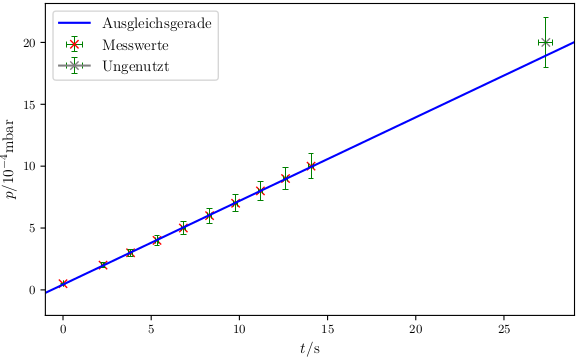
\includegraphics[width=\linewidth-70pt,height=\textheight-70pt,keepaspectratio]{content/images/TL4.png}
\caption{Der Druck $p$ in Abhängigkeit von der mittleren Zeit $\bar{t}$ bei der Leckratenmessung der Turbopumpe  mit $p_g = \SI{0.5e-4}{\milli\bar}$.}
\label{fig:TL4}
\end{figure}

\subsubsection{Bestimmung des Saugvermögens $S$ über die Evakuierungskurve}

In Tabelle \ref{tab:TS} sind die Messwerte für die Evakuierungskurve, sowie die nach Formel \eqref{eq:tQuer} berechneten Mittelwerte $\bar{t}$ eingetragen.
Dabei entsprechen $p_0=\SI{500(100)e-5}{\milli\bar}$ dem Anfangsdruck und $p_e=\SI{1.2(2)e-5}{\milli\bar}$ dem Enddruck der Kurve. Der Fehler des Druckes ergibt sich aus der Ungenauigkeit der Messskala von $20\%$ \cite{V70}. 
Der Fehler der logarithmischen Werte berechnet sich nach der Gaußschen Fehlerfortpflanzung:
\[
\sigma_f = \sqrt{\sum_i\left(\frac{\partial f}{\partial x_i}\sigma_{x_i}\right)^2}\text{.}
\]
Konkret:
\begin{align*}
\sigma_.{ln}	&=\sqrt{\frac{\sigma_p^2+\sigma_{p_e}^2}{(p-p_e)^2}+\frac{\sigma_{p_0}^2+\sigma_{p_e}^2}{(p_0-p_e)^2}}\text{.}
%\sigma_.{ln}	&=\frac{1}{z}\sigma_{z}\text{;}\\
%z				&=\frac{p-p_e}{p_0-p_e}\text{,}\\
%\sigma_{z}	&=\sqrt{\left(\frac{1}{p_y}\sigma_{p_x}\right)^2+\left(\frac{p_x}{p_y^2}\sigma_{p_y}\right)^2}\text{;}\\
%p_x				&=p-p_e\text{,}\\
%p_y				&=p_0-p_e\text{,}\\
%\sigma_{p_x}	&=\sqrt{\sigma_p^2+\sigma_{p_e}^2}\text{,}\\
%\sigma_{p_y}	&=\sqrt{\sigma_{p_0}^2+\sigma_{p_e}^2}\text{.}\\
\end{align*}
Dabei entsprechen die $\sigma_{p_i}$ den jeweiligen Abweichungen der $p_i$.
Die Evakuierungskurve ist in Abbildung \ref{fig:TSE} zu sehen, die logarithmische Darstellung in Abbildung \ref{fig:TSL}.
Lineare Ausgleichsrechnungen der Form
\[
\ln\left(\frac{p(t)-p_e}{p_0-p_e}\right) = a_it+b_i
\]
für die ersten vier Messwerte (Ausgleichsgerade 1), den fünften bis achten Messwert (Ausgleichsgerade 2) und den siebten bis zehnten Messwert (Ausgleichsgerade 3) ergeben die Parameter:
\begin{align*}
a_.{TE1} &= \SI{-0.89(2)}{\per\second} \text{,}\\
b_.{TE1} &= \SI{-0.05(5)}{} \text{,}\\
a_.{TE2} &= \SI{-0.51(4)}{\per\second} \text{,}\\
b_.{TE2} &= \SI{-1.9(3)}{} \text{,}\\
a_.{TE3} &= \SI{-0.21(3)}{\per\second} \text{,}\\
b_.{TE3} &= \SI{-4.6(3)}{} \text{.}\\
\end{align*} 
Daraus folgen mit Formel \eqref{eq:} für $S$ die Werte:
\begin{align*}
S_.{TE1} &= \SI{9.1(8)}{\litre\per\second} \text{,}\\
S_.{TE2} &= \SI{5.2(6)}{\litre\per\second} \text{,}\\
S_.{TE3} &= \SI{2.2(3)}{\litre\per\second} \text{.}\\
\end{align*} 
Das benötigte Volumen $V_.{TE}$ bestimmt sich dabei mit den Werten aus \ref{tab:V} zu:
\[
V_.{TE} = \dots = \SI{10.3(9)}{\litre}\text{.}
\]

\begin{table}
\centering
\caption{Die Werte für die Evakuierungskurve der Turborpumpe.}
\label{tab:tabTS}
	\sisetup{table-format=1.2}
	\begin{tabular}{S[table-format=3.1] @{${}\pm{}$} S[table-format=2.1]S[table-format=2.1] @{${}\pm{}$} S[table-format=1.1]S[table-format=2.2]S[table-format=2.2]S[table-format=2.2]S[table-format=2.2]S[table-format=2.2]S[table-format=2.2]S[table-format=2.2] @{${}\pm{}$} S[table-format=1.2]}
		\toprule
		\multicolumn{2}{c}{$p/10^{-5}\si{\milli\bar}$} & \multicolumn{2}{c}{$\log\left(\frac{p-p_e}{p_0-p_e}\right)$} & {$t_1/\si{\second}$} & {$t_2/\si{\second}$} & {$t_3/\si{\second}$} & {$t_4/\si{\second}$} & {$t_5/\si{\second}$} & {$t_6/\si{\second}$} & \multicolumn{2}{c}{$\bar{t}/\si{\second}$} \\
		\midrule
		500.0 & 50.0 & 0.0 & 0.0 & 0.00 & 0.00 & 0.00 & 0.00 & 0.00 & 0.00 & 0.00 & 0.00 \\
		200.0 & 20.0 & -0.9 & 0.2 & 0.86 & 0.98 & 0.90 & 0.93 & 0.81 & 1.03 & 0.92 & 0.04 \\
		40.0 & 4.0 & -2.6 & 0.2 & 2.72 & 2.82 & 2.71 & 2.89 & 2.71 & 2.98 & 2.81 & 0.05 \\
		20.0 & 2.0 & -3.3 & 0.2 & 3.57 & 3.78 & 3.51 & 3.80 & 3.54 & 3.84 & 3.67 & 0.07 \\
		6.0 & 0.6 & -4.6 & 0.2 & 5.55 & 5.69 & 5.50 & 5.66 & 5.47 & 5.82 & 5.61 & 0.06 \\
		4.0 & 0.4 & -5.2 & 0.2 & 6.31 & 6.48 & 6.28 & 6.69 & 6.31 & 6.60 & 6.45 & 0.08 \\
		2.0 & 0.2 & -6.4 & 0.4 & 8.66 & 8.89 & 8.71 & 8.75 & 8.69 & 9.18 & 8.81 & 0.09 \\
		1.8 & 0.2 & -6.7 & 0.4 & 9.82 & 9.80 & 9.76 & 9.66 & 9.40 & 10.24 & 9.78 & 0.12 \\
		1.6 & 0.2 & -7.1 & 0.6 & 11.01 & 11.13 & 11.34 & 10.64 & 10.56 & 11.40 & 11.01 & 0.15 \\
		1.4 & 0.2 & -7.8 & 1.0 & 15.24 & 15.19 & 15.34 & 14.85 & 14.59 & 15.45 & 15.11 & 0.14 \\
		\bottomrule
	\end{tabular}

\label{tab:TS}
\end{table}

\begin{figure}
\centering
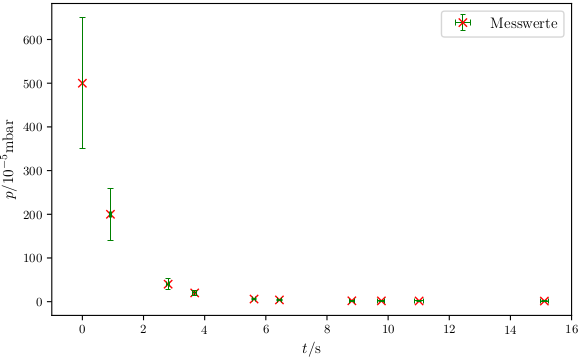
\includegraphics[width=\linewidth-70pt,height=\textheight-70pt,keepaspectratio]{content/images/TSE.png}
\caption{Die Evakuierungskurve der Turbopumpe.}
\label{fig:TSE}
\end{figure}

\begin{figure}
\centering
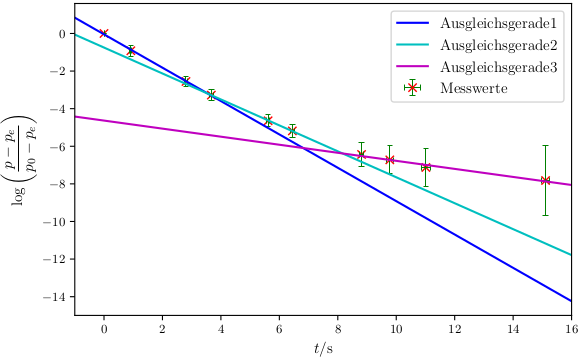
\includegraphics[width=\linewidth-70pt,height=\textheight-70pt,keepaspectratio]{content/images/TSL.png}
\caption{Die logarithmische Evakuierungskurve der Turbopumpe.}
\label{fig:TSL}
\end{figure}

\subsection{Drehschieberpumpe}

\subsubsection{Bestimmung des Saugvermögens $S$ über die Leckratenmessung}

Die Leckratenmessung wurde bei vier unterschiedlichen Gleichgewichtsdrücken $p_g$ durchgeführt. Dabei werden die gemessenen Zeiten $t_i$ mit Formel \eqref{eq:tQuer} gemittelt.
In den Tabellen \ref{tab:DL1} bis \ref{tab:DL4} sind die Messwerte und die zugehörigen Mittelwerte der jeweiligen Messreihen aufgelistet. Der Fehler des Druckes ergibt sich dabei aus der Ungenauigkeit der Messskala von $10\%$ \cite{V70}.\\
In den Abbildungen \ref{fig:DL1} bis \ref{fig:DL4} ist der Druck $p$ gegen die gemittelte Zeit $\bar{t}$ aufgetragen.
Die linearen Ausgleichsrechnungen der Form
\[
p_i(t) = a_it+b_i
\]
ergeben für $p_g = \SI{1}{\milli\bar}$ die Parameter
\begin{align*}
a_.{DL1} &= \SI{0.122(2)}{\milli\bar\per\second} \text{,}\\
b_.{DL1} &= \SI{0.91(6)}{\milli\bar} \text{,}\\
\end{align*}
für $p_g = \SI{0.8}{\milli\bar}$
\begin{align*}
a_.{DL2} &= \SI{0.098(2)}{\milli\bar\per\second} \text{,}\\
b_.{DL2} &= \SI{0.77(6)}{\milli\bar} \text{,}\\
\end{align*}
für $p_g = \SI{0.4}{\milli\bar}$
\begin{align*}
a_.{DL3} &= \SI{0.034(1)}{\milli\bar\per\second} \text{,}\\
b_.{DL3} &= \SI{0.25(9)}{\milli\bar} \text{,}\\
\end{align*}
und für $p_g = \SI{0.1}{\milli\bar}$
\begin{align*}
a_.{DL4} &= \SI{0.0048(2)}{\milli\bar\per\second} \text{,}\\
b_.{DL4} &= \SI{0.14(2)}{\milli\bar} \text{.}
\end{align*}
In denGraphen sind die nicht genutzten Messwerte Grau markiert.
Mit Formel \eqref{eq:S2} ergibt sich für das Saugvermögen $S$
\begin{align*}
S_.{DL1} &= \SI{1.4(1)}{\litre\per\second} \text{,}\\
S_.{DL2} &= \SI{1.4(1)}{\litre\per\second} \text{,}\\
S_.{DL3} &= \SI{0.95(9)}{\litre\per\second} \text{,}\\
S_.{DL4}   &= \SI{0.53(5)}{\litre\per\second} \text{.}
\end{align*}
Das benötigte Volumen $V_.{DL}$ bestimmt sich dabei mit den Werten aus \ref{tab:V} zu:
\[
V_.{DL} = \dots = \SI{11(1)}{\litre}\text{.}
\]


\begin{table}
\centering
\caption{Die Messwerte der Leckratenmessung bei der Drehschieberpumpe mit einem Gleichgewichtsdruck von $p_g = \SI{1}{\milli\bar}$.}
\label{tab:tabDL1}
	\sisetup{table-format=1.2}
	\begin{tabular}{S[table-format=2.0] @{${}\pm{}$} S[table-format=1.1]S[table-format=2.2]S[table-format=2.2]S[table-format=2.2]S[table-format=2.2]S[table-format=2.2] @{${}\pm{}$} S[table-format=1.2]}
		\toprule
		\multicolumn{2}{c}{$p/\si{\milli\bar}$} & {$t_1/\si{\second}$} & {$t_2/\si{\second}$} & {$t_3/\si{\second}$} & {$t_4/\si{\second}$} & \multicolumn{2}{c}{$\bar{t}/\si{\second}$} \\
		\midrule
		 2 & 0.4 & 8.91 & 9.81 & 10.36 & 9.55 & 9.66 & 0.30 \\
		 4 & 0.8 & 25.87 & 25.15 & 27.01 & 26.21 & 26.06 & 0.39 \\
		 6 & 1.2 & 40.78 & 41.33 & 42.06 & 40.74 & 41.23 & 0.31 \\
		 8 & 1.6 & 57.78 & 58.09 & 56.92 & 57.58 & 57.59 & 0.25 \\
		10 & 2.0 & 74.33 & 75.40 & 76.27 & 73.51 & 74.88 & 0.60 \\
		\bottomrule
	\end{tabular}

\label{tab:DL1}
\end{table}

\begin{figure}
\centering
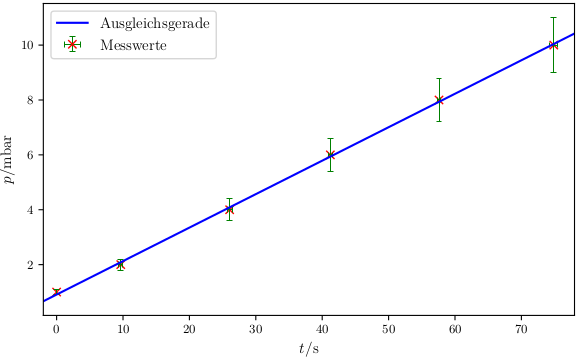
\includegraphics[width=\linewidth-70pt,height=\textheight-70pt,keepaspectratio]{content/images/DL1.png}
\caption{Der Druck $p$ in Abhängigkeit von der mittleren Zeit $\bar{t}$ bei der Leckratenmessung der Drehschieberpumpe  mit $p_g = \SI{1}{\milli\bar}$.}
\label{fig:DL1}
\end{figure}

\begin{table}
\centering
\caption{Die Messwerte der Leckratenmessung bei der Drehschieberpumpe mit einem Gleichgewichtsdruck von $p_g = \SI{0.8}{\milli\bar}$.}
\label{tab:tabDL2}
	\sisetup{table-format=1.2}
	\begin{tabular}{S[table-format=2.0] @{${}\pm{}$} S[table-format=1.1]S[table-format=2.2]S[table-format=2.2]S[table-format=2.2]S[table-format=2.2] @{${}\pm{}$} S[table-format=1.2]}
		\toprule
		\multicolumn{2}{c}{$p/\si{\milli\bar}$} & {$t_1/\si{\second}$} & {$t_2/\si{\second}$} & {$t_3/\si{\second}$} & \multicolumn{2}{c}{$\bar{t}/\si{\second}$} \\
		\midrule
		 2 & 0.4 & 12.28 & 11.88 & 12.29 & 12.15 & 0.14 \\
		 4 & 0.8 & 33.98 & 35.09 & 33.67 & 34.25 & 0.44 \\
		 6 & 1.3 & 52.83 & 52.47 & 52.65 & 52.65 & 0.11 \\
		 8 & 1.6 & 73.54 & 73.97 & 73.18 & 73.56 & 0.23 \\
		10 & 2.0 & 76.73 & 76.87 & 75.98 & 76.53 & 0.28 \\
		\bottomrule
	\end{tabular}

\label{tab:DL2}
\end{table}

\begin{figure}
\centering
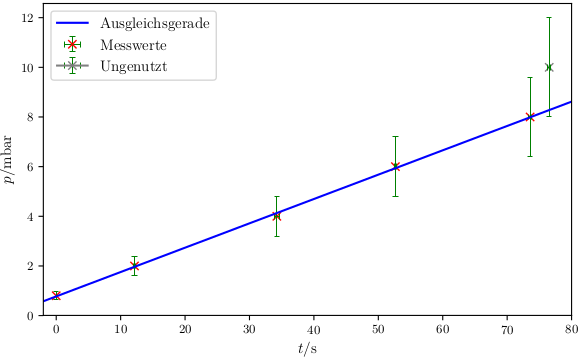
\includegraphics[width=\linewidth-70pt,height=\textheight-70pt,keepaspectratio]{content/images/DL2.png}
\caption{Der Druck $p$ in Abhängigkeit von der mittleren Zeit $\bar{t}$ bei der Leckratenmessung der Drehschieberpumpe  mit $p_g = \SI{0.8}{\milli\bar}$.}
\label{fig:DL2}
\end{figure}

\begin{table}
\centering
\caption{Die Messwerte der Leckratenmessung bei der Drehschieberpumpe mit einem Gleichgewichtsdruck von $p_g = \SI{0.4}{\milli\bar}$.}
\label{tab:tabDL3}
	\sisetup{table-format=1.2}
	\begin{tabular}{S[table-format=1.1] @{${}\pm{}$} S[table-format=1.1]S[table-format=2.2]S[table-format=2.2]S[table-format=2.2]S[table-format=2.2] @{${}\pm{}$} S[table-format=1.2]}
		\toprule
		\multicolumn{2}{c}{$p/\si{\milli\bar}$} & {$t_1/\si{\second}$} & {$t_2/\si{\second}$} & {$t_3/\si{\second}$} & \multicolumn{2}{c}{$\bar{t}/\si{\second}$} \\
		\midrule
		0.6 & 0.1 & 8.28 & 9.35 & 8.71 & 8.78 & 0.31 \\
		1.0 & 0.1 & 23.33 & 23.89 & 23.85 & 23.69 & 0.18 \\
		2.0 & 0.2 & 57.47 & 56.65 & 55.97 & 56.70 & 0.43 \\
		4.0 & 0.4 & 113.70 & 113.33 & 112.68 & 113.24 & 0.30 \\
		6.0 & 0.6 & 164.21 & 165.51 & 165.13 & 164.95 & 0.39 \\
		\bottomrule
	\end{tabular}

\label{tab:DL3}
\end{table}

\begin{figure}
\centering
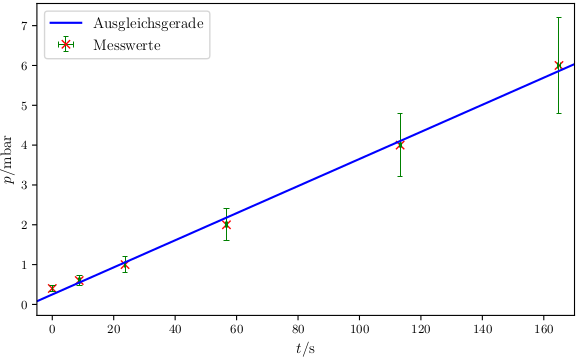
\includegraphics[width=\linewidth-70pt,height=\textheight-70pt,keepaspectratio]{content/images/DL3.png}
\caption{Der Druck $p$ in Abhängigkeit von der mittleren Zeit $\bar{t}$ bei der Leckratenmessung der Drehschieberpumpe  mit $p_g = \SI{0.4}{\milli\bar}$.}
\label{fig:DL3}
\end{figure}

\begin{table}
\centering
\caption{Die Messwerte der Leckratenmessung bei der Drehschieberpumpe mit einem Gleichgewichtsdruck von $p_g = \SI{0.1}{\milli\bar}$.}
\label{tab:tabDL4}
	\sisetup{table-format=1.2}
	\begin{tabular}{S[table-format=1.1] @{${}\pm{}$} S[table-format=1.2]S[table-format=2.2]S[table-format=2.2]S[table-format=2.2]S[table-format=2.2] @{${}\pm{}$} S[table-format=1.2]}
		\toprule
		\multicolumn{2}{c}{$p/\si{\milli\bar}$} & {$t_1/\si{\second}$} & {$t_2/\si{\second}$} & {$t_3/\si{\second}$} & \multicolumn{2}{c}{$\bar{t}/\si{\second}$} \\
		\midrule
		0.2 & 0.05 & 9.95 & 10.08 & 10.66 & 10.23 & 0.22 \\
		0.4 & 0.09 & 46.08 & 46.54 & 46.48 & 46.37 & 0.15 \\
		0.6 & 0.12 & 93.01 & 95.29 & 95.11 & 94.47 & 0.74 \\
		0.8 & 0.17 & 141.51 & 141.29 & 142.19 & 141.66 & 0.28 \\
		1.0 & 0.20 & 179.62 & 180.72 & 180.07 & 180.14 & 0.32 \\
		\bottomrule
	\end{tabular}

\label{tab:DL4}
\end{table}

\begin{figure}
\centering
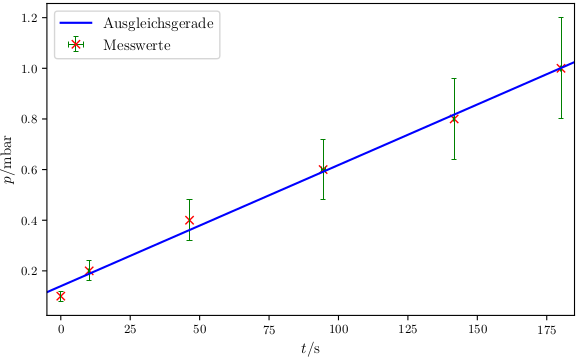
\includegraphics[width=\linewidth-70pt,height=\textheight-70pt,keepaspectratio]{content/images/DL4.png}
\caption{Der Druck $p$ in Abhängigkeit von der mittleren Zeit $\bar{t}$ bei der Leckratenmessung der Drehschieberpumpe  mit $p_g = \SI{0.1}{\milli\bar}$.}
\label{fig:DL4}
\end{figure}

\subsubsection{Bestimmung des Saugvermögens $S$ über die Evakuierungskurve}

In Tabelle \ref{tab:DS} sind die Messwerte für die Evakuierungskurve, sowie die nach Formel \eqref{eq:tQuer} berechneten Mittelwerte $\bar{t}$ eingetragen.
Dabei entsprechen $p_0=\SI{1013}{\milli\bar}$ dem Anfangsdruck und $p_e=\SI{0.02}{\milli\bar}$ dem Enddruck der Kurve. Der Fehler des Druckes ergibt sich aus der Ungenauigkeit der Messskala von $20\%$ \cite{V70}. 
Der Fehler der logarithmischen Werte berechnet sich nach Formel \eqref{}.
Die Evakuierungskurve ist in Abbildung \ref{fig:DSE} zu sehen, die logarithmische Darstellung in Abbildung \ref{fig:DSL}.
Lineare Ausgleichsrechnungen der Form
\[
\ln\left(\frac{p(t)-p_e}{p_0-p_e}\right) = a_it+b_i
\]
für die ersten elf Messwerte (Ausgleichsgerade 1) und den zwöften bis siebzehnten Messwert (Ausgleichsgerade 2) ergeben die Parameter:
\begin{align*}
a_.{DE1} &= \SI{-0.093(2)}{\per\second} \text{,}\\
b_.{DE1} &= \SI{-0.08(8)}{} \text{,}\\
a_.{DE2} &= \SI{-0.0619(8)}{\per\second} \text{,}\\
b_.{DE2} &= \SI{-2.51(8)}{} \text{,}\\
\end{align*} 
Daraus folgen mit Formel \eqref{eq:} für $S$ die Werte:
\begin{align*}
S_.{DE1} &= \SI{1.0(1)}{\litre\per\second} \text{,}\\
S_.{DE2} &= \SI{0.69(6)}{\litre\per\second} \text{.}\\
\end{align*} 
Das benötigte Volumen $V_.{TE}$ bestimmt sich dabei mit den Werten aus \ref{tab:V} zu:
\[
V_.{DE} = \dots = \SI{11.1(1)}{\litre}\text{.}
\]

\begin{table}
\centering
\caption{Die Werte für die Evakuierungskurve der Drehschieberpumpe.}
\label{tab:tabDS}
	\sisetup{table-format=1.2}
	\begin{tabular}{S[table-format=3.2] @{${}\pm{}$} S[table-format=2.2]S[table-format=3.1] @{${}\pm{}$} S[table-format=1.1]S[table-format=3.2]S[table-format=3.2]S[table-format=3.2]S[table-format=3.2]S[table-format=3.2]S[table-format=3.2]@{${}\pm{}$} S[table-format=1.2]}
		\toprule
		\multicolumn{2}{c}{$p/\si{\milli\bar}$} & \multicolumn{2}{c}{$\log\left(\frac{p-p_e}{p_0-p_e}\right)$} & {$t_1/\si{\second}$} & {$t_2/\si{\second}$} & {$t_3/\si{\second}$} & {$t_4/\si{\second}$} & {$t_5/\si{\second}$} & \multicolumn{2}{c}{$\bar{t}/\si{\second}$} \\
		\midrule
		100.00 & 20.00 & -2.3 & 0.3 & 18.81 & 21.62 & 21.50 & 21.49 & 22.65 & 21.21 & 0.64 \\
		60.00 & 12.00 & -2.8 & 0.3 & 28.25 & 30.40 & 29.56 & 29.04 & 29.66 & 29.38 & 0.36 \\
		40.00 & 8.00 & -3.2 & 0.3 & 34.20 & 35.60 & 34.94 & 34.60 & 35.09 & 34.89 & 0.24 \\
		20.00 & 4.00 & -3.9 & 0.3 & 41.58 & 42.91 & 42.67 & 42.14 & 42.74 & 42.41 & 0.24 \\
		10.00 & 2.00 & -4.6 & 0.3 & 48.64 & 50.71 & 50.13 & 49.57 & 50.15 & 49.84 & 0.35 \\
		8.00 & 1.60 & -4.8 & 0.3 & 51.02 & 52.75 & 52.53 & 51.62 & 52.26 & 52.04 & 0.32 \\
		6.00 & 1.20 & -5.1 & 0.3 & 54.26 & 55.95 & 55.67 & 55.18 & 55.54 & 55.32 & 0.29 \\
		4.00 & 0.80 & -5.5 & 0.3 & 57.89 & 59.43 & 59.56 & 58.78 & 59.44 & 59.02 & 0.31 \\
		2.00 & 0.40 & -6.2 & 0.3 & 64.57 & 66.21 & 66.08 & 65.64 & 66.19 & 65.74 & 0.31 \\
		1.00 & 0.20 & -6.9 & 0.3 & 71.90 & 73.67 & 73.49 & 73.12 & 73.60 & 73.16 & 0.33 \\
		0.80 & 0.16 & -7.2 & 0.3 & 74.34 & 75.85 & 76.00 & 75.51 & 75.98 & 75.54 & 0.31 \\
		0.60 & 0.12 & -7.5 & 0.3 & 78.49 & 80.16 & 80.20 & 79.46 & 80.18 & 79.70 & 0.33 \\
		0.40 & 0.08 & -7.9 & 0.3 & 85.43 & 87.42 & 86.81 & 86.62 & 87.16 & 86.69 & 0.34 \\
		0.20 & 0.04 & -8.6 & 0.3 & 98.56 & 99.93 & 99.71 & 99.35 & 99.56 & 99.42 & 0.24 \\
		0.10 & 0.02 & -9.4 & 0.3 & 110.69 & 111.87 & 111.74 & 110.95 & 111.57 & 111.36 & 0.23 \\
		0.08 & 0.02 & -9.7 & 0.3 & 116.74 & 117.48 & 116.94 & 116.99 & 116.93 & 117.02 & 0.12 \\
		0.06 & 0.01 & -10.1 & 0.4 & 129.17 & 129.04 & 128.40 & 127.59 & 128.66 & 128.57 & 0.28 \\
		\bottomrule
	\end{tabular}

\label{tab:DS}
\end{table}

\begin{figure}
\centering
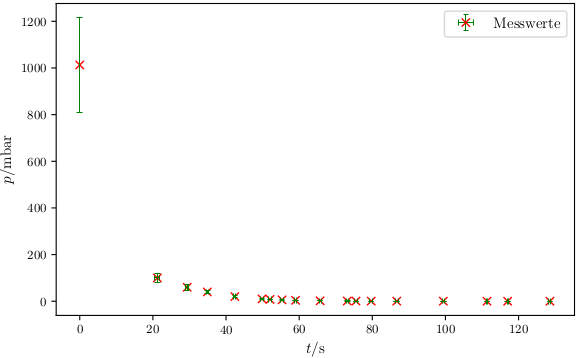
\includegraphics[width=\linewidth-70pt,height=\textheight-70pt,keepaspectratio]{content/images/DSE.png}
\caption{Die Evakuierungskurve der Drehschieberpumpe.}
\label{fig:DSE}
\end{figure}

\begin{figure}
\centering
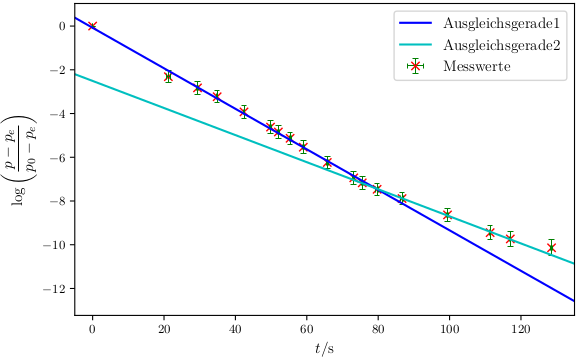
\includegraphics[width=\linewidth-70pt,height=\textheight-70pt,keepaspectratio]{content/images/DSL.png}
\caption{Die logarithmische Evakuierungskurve der Drehschieberpumpe.}
\label{fig:DSL}
\end{figure}

\subsection{Zusammenfassung}

\begin{figure}
\centering
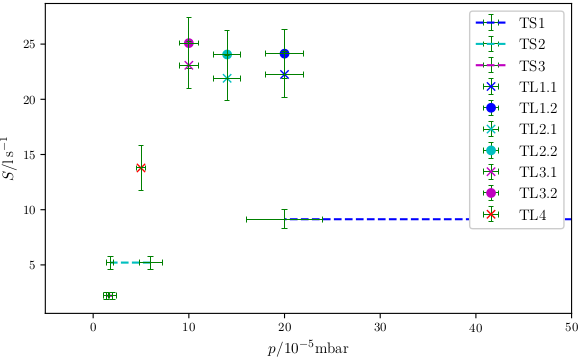
\includegraphics[width=\linewidth-70pt,height=\textheight-70pt,keepaspectratio]{content/images/TGes.png}
\caption{Das Saugvermögen $S$ der Turbomoolekularpumpe in Abhängigkeit vom Druck $p$.}
\label{fig:TGes}
\end{figure}

\begin{figure}
\centering
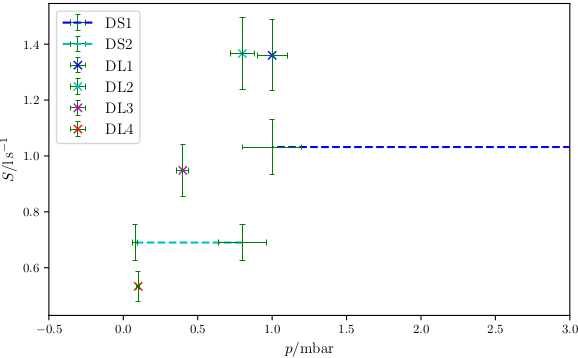
\includegraphics[width=\linewidth-70pt,height=\textheight-70pt,keepaspectratio]{content/images/DGes.png}
\caption{Das Saugvermögen $S$ der Drehschieberpumpe in Abhängigkeit vom Druck $p$.}
\label{fig:DGes}
\end{figure}
	
\section{Diskussion}
\label{sec:Diskussion}

Die Werte des magnetischen Moments sind bei den ersten beiden Messreihen nahezu identisch, was darauf schließen lässt, dass diese sehr nah am wirklichen Wert liegen. Dies wird durch die geringen Fehler unterstützt. Dabei ist die zweite Methode leichter durchzuführen, da hier das Magnetfeld nicht so präzise wie bei der ersten Methode eingestellt werden muss. Der Fehler, der durch das ungenaue Messen der Periodendauer zustande kommt, wird dabei durch Messung mehrerer Periodendauern und anschließendem mitteln kompensiert.\newline 
Wie zu erwarten, weicht das Ergebnis der dritten Messung von den anderen beiden ab. Dies liegt daran, dass hier die meisten Messfehler gemacht werden können. Die Frequenz ist nur schwer auf den vorgegebenen Wert zu bringen und nimmt während der Präzession zu schnell ab. Zudem kann die Präzessionsdauer nur befriedigend genau bestimmt werden, welches an den teilweise größeren Abweichungen dieser Werte zu erkennen ist. Das Ergebnis dieser Messung könnte durch längere und häufigere Messungen verbessert werden. Zudem könnte durch ein besseres Luftkissen die Abnahme der Frequenz verringert werden. 
	\newpage
	\printbibliography[title=Literatur]
\end{document}